\documentclass{beamer}
\usepackage[utf8]{inputenc}
\usepackage[T1]{fontenc}
\usepackage[french]{babel}
\usetheme{Hannover}
\usecolortheme{crane}
\usefonttheme{serif}
\usepackage{listings}
\usepackage{multicol}
\usepackage{fixltx2e}

\definecolor{black}{RGB}{0,0,0}
\definecolor{mygreen}{rgb}{0,0.6,0}
\definecolor{myorange}{rgb}{1.0,0.6,0.0}
\definecolor{mygray}{rgb}{0.5,0.5,0.5}
\definecolor{mymauve}{rgb}{0.58,0,0.82}
\lstset{%
  identifierstyle=\color{myorange},
  backgroundcolor=\color{white},   % choose the background color; you must add \usepackage{color} or \usepackage{xcolor}
  basicstyle=\scriptsize,        % the size of the fonts that are used for the code
  breakatwhitespace=false,         % sets if automatic breaks should only happen at whitespace
  breaklines=true,                 % sets automatic line breaking
  captionpos=b,                    % sets the caption-position to bottom
  commentstyle=\color{mygreen},    % comment style
  extendedchars=true,              % lets you use non-ASCII characters; for 8-bits encodings only, does not work with UTF-8
  frame=single,                    % adds a frame around the code
  keepspaces=true,                 % keeps spaces in text, useful for keeping indentation of code (possibly needs columns=flexible)
  keywordstyle=\color{blue},       % keyword style
  morekeywords={}, % if you want to add more keywords to the set
  numbers=left,                    % where to put the line-numbers; possible values are (none, left, right)
  numbersep=5pt,                   % how far the line-numbers are from the code
  numberstyle=\tiny\color{mygray}, % the style that is used for the line-numbers
  rulecolor=\color{black},         % if not set, the frame-color may be changed on line-breaks within not-black text (e.g. comments (green here))
  showspaces=false,                % show spaces everywhere adding particular underscores; it overrides 'showstringspaces'
  showstringspaces=false,          % underline spaces within strings only
  showtabs=false,                  % show tabs within strings adding particular underscores
  stepnumber=1,                    % the step between two line-numbers. If it's 1, each line will be numbered
  stringstyle=\color{mymauve},     % string literal style
  tabsize=2,                       % sets default tabsize to 2 spaces
  title=\lstname                   % show the filename of files included with \lstinputlisting; also try caption instead of title
}

\AtBeginSubsection[]{%
\begin{frame}<beamer>{Table of Contents}
  \begin{multicols}{2}
\tableofcontents[currentsection,currentsubsection,
    hideothersubsections,
    sectionstyle=show/shaded,
    subsectionstyle=show/shaded,
]
  \end{multicols}
\end{frame}
}

\begin{document}

\title{GNU Bison}
\author{Theophile Ranquet
Valentin Tolmer}
\institute{%
  Ecole Pour l'Informatique et les Techniques Avancées\\
  \texttt{ranquet@lrde.epita.fr}\\
  \texttt{nitnelave1@gmail.com}
}

\date{December 17, 2013}

\begin{frame}[plain]
  \titlepage
\end{frame}

\begingroup
\setbeamercolor{background canvas}{bg=craneorange!90}
\begin{frame}
    \begin{center}
        \vspace{1cm}
        {\Huge\color{black} \textbf{1.} {\fontencoding{T1}\fontfamily{anttlc}\fontseries{m}\fontshape{n} Parsers}}
    \end{center}
\end{frame}
\endgroup

\section{Parsers}

\subsection{Grammars and parsers}

\begin{frame}
  \frametitle{What is a parser?}
  \textbf{Parsing}, or \textbf{syntactic analysis} is the process of analysing
  a string of symbols, either in natural language or in computer languages,
  according to the rules of a formal grammar.

  \vfill

  A parser is a software component that takes \textbf{input} data (frequently
  text) and builds a data structure – often some kind of parse tree, abstract
  syntax tree or other hierarchical structure, \textbf{checking} for correct
  syntax in the process.

\end{frame}
\begin{frame}
  The parser is often preceded by a separate \textbf{lexical analyser}, which
  creates tokens from the sequence of input characters; alternatively, these
  can be combined in scannerless parsing.

  \vfill

  Parsers may be programmed by hand or may be automatically or
  semi-automatically generated by a parser generator.

  \vfill

  Parsing is complementary to \textit{templating}, which produces formatted output.
  These may be applied to different domains, but often appear together, such as
  the \texttt{scanf/printf} pair, or the input (front end parsing) and output
  (back end code generation) stages of a \textbf{compiler}.
\end{frame}

\begin{frame}
  \frametitle{Parsing and lexing}
  \begin{center}
    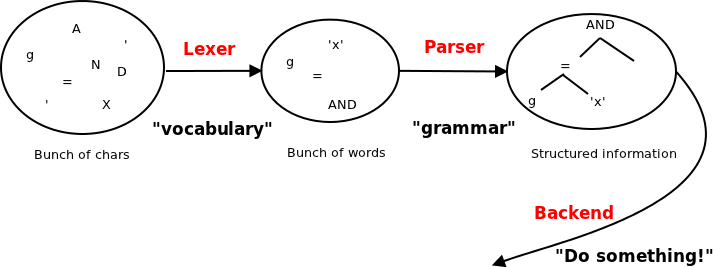
\includegraphics[scale=0.4]{lexer_parser}
  \end{center}
\end{frame}

\begin{frame}
  \frametitle{Grammars and types of parsers}

  An important class of simple parsing is done using \textbf{regular
  expressions}, where a regular expression defines a \textbf{regular language},
  and then the regular expression engine automatically generates a parser for
  that language, allowing pattern matching and extraction of text. In other
  contexts regular expressions are instead used prior to parsing, as the
  \textbf{lexing} step whose output is then used by the parser.

  \vfill

  Programming languages tend to be specified in terms of a deterministic
  context-free grammar because fast and efficient parsers can be written for
  them.
\end{frame}

\begin{frame}
  \frametitle{Context-sensitivity}

  \textbf{Context-free grammars} are limited in the extent to which they can
  express all of the requirements of a language, because they have limited
  \textit{memory}: for example, if a name must be declared before it may be
  referenced.

  \vfill

  Thus, it is a common strategy to create a relaxed parser for a context-free
  grammar which accepts a superset of the desired language constructs (that is,
  it accepts some invalid constructs); later, the unwanted constructs can be
  filtered out at the \textbf{semantic analysis} (contextual analysis) step.
\end{frame}

\begin{frame}[fragile]
  For example, in \textbf{Python} the following is \textit{syntactically} valid
  code:

  \begin{lstlisting}[language=python]
  x = 1
  print x \end{lstlisting}

  The following code, however, is syntactically valid in terms of the
  \textbf{context-free} grammar, yielding a syntax tree with the same structure
  as the previous, but is syntactically \textit{invalid} in terms of the
  \textbf{context-sensitive} grammar, which requires that variables be
  initialized before use:

  \begin{lstlisting}[language=python]
  x = 1
  print y \end{lstlisting}

  Rather than being analyzed at the parsing stage, this is caught by checking
  the values in the syntax tree, hence as part of \textbf{semantic analysis}:
  context-sensitive syntax is in practice often more easily analyzed as
  semantics.
\end{frame}

\begin{frame}
  \frametitle{Compiler design}
  \begin{center}
    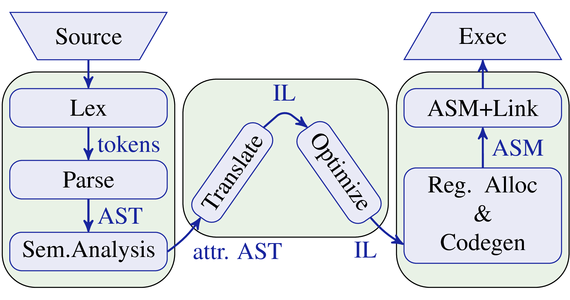
\includegraphics[scale=0.5]{compiler}
  \end{center}
\end{frame}

\begin{frame}
  \frametitle{Types of parsers}
There are (essentially) two ways to parse:
\begin{itemize}
  \item \textbf{Top-down} parsing can be viewed as an attempt to find left-most
derivations of an input-stream by searching for parse trees using a top-down
expansion of the given formal grammar rules. Tokens are consumed from left to
right. \textbf{LL} (\textbf{L}eft-to-Right, \textbf{L}eftmost derivation)
parsers are an example of such parsers.

  \item \textbf{Bottom-up} (or \textit{Shift/Reduce}) parsing starts with the
input and attempts to rewrite it to the start symbol.  Intuitively, the parser
attempts to locate the most basic elements, then the elements containing these,
and so on. \textbf{LR} (\textbf{L}eft-to-right, \textbf{R}ightmost derivation)
parsers are examples of bottom-up parsers.
\end{itemize}
\end{frame}

\begin{frame}
  \frametitle{LL vs LR}
  \begin{center}
    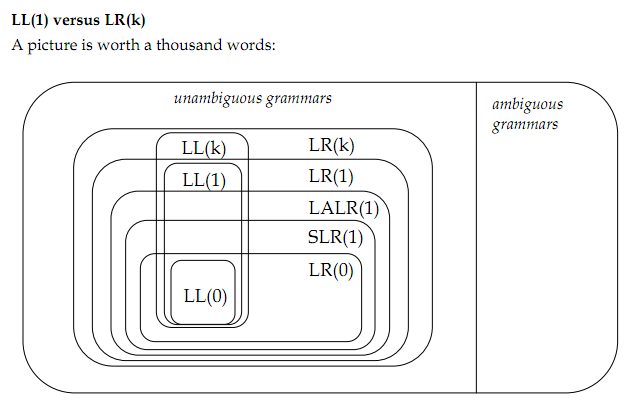
\includegraphics[scale=0.47]{LLLR}
  \end{center}
\end{frame}

\begin{frame}
  \frametitle{Top-down vs bottom-up}
  \begin{center}
    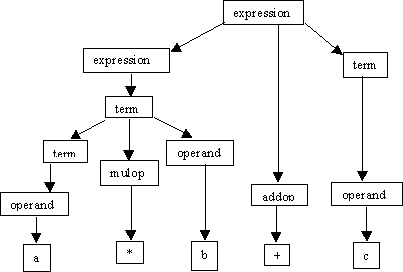
\includegraphics[scale=0.3]{topdown}
\hfill
    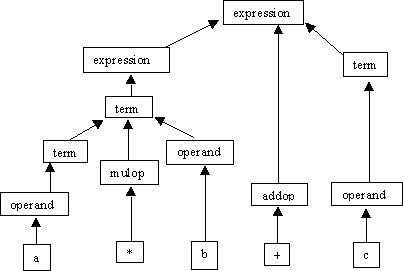
\includegraphics[scale=0.3]{bottomup}
  \end{center}
\end{frame}

\begin{frame}
  \frametitle{Top-down parsing}
  \begin{center}
    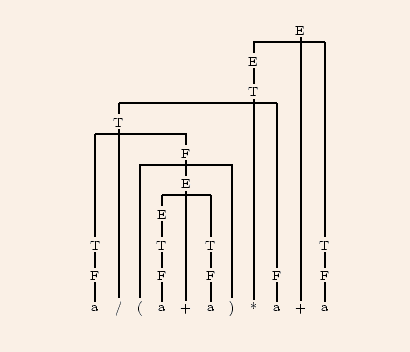
\includegraphics[scale=0.3]{topdown2}
  \end{center}
\end{frame}

\begin{frame}
  \frametitle{Bottom-up parsing}
  \begin{center}
    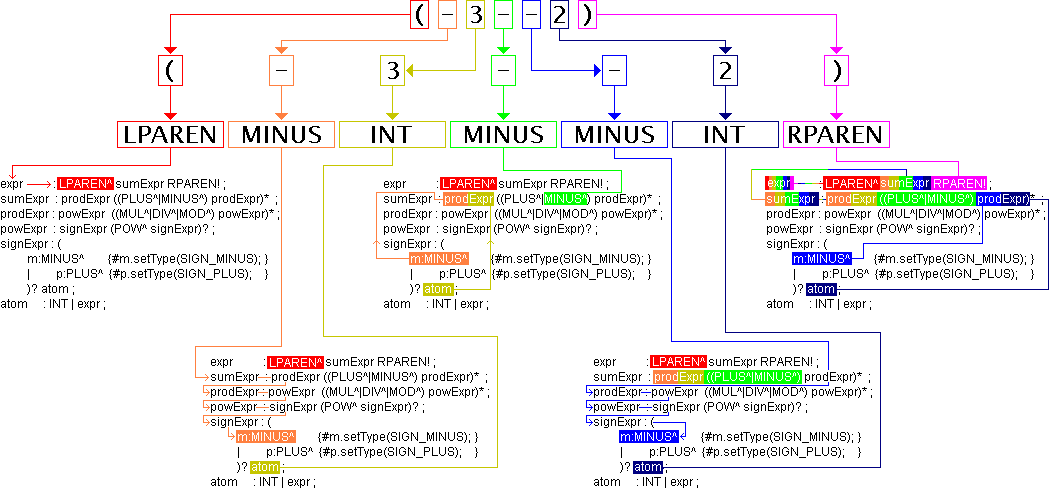
\includegraphics[scale=0.3]{sillyastthing}
  \end{center}
\end{frame}

\begin{frame}
  \frametitle{Lookahead parsing}
  \textbf{Lookahead} establishes the maximum incoming tokens that a parser can
  use to decide which rule it should use.  It is often explicitly indicated by
  affixing the lookahead to the algorithm name in parentheses, such as LALR(1)

  \vfill

Lookahead has two advantages:
\begin{itemize}
  \item It helps the parser take the correct action in case of
    \textbf{conflicts}. For example, parsing the \texttt{if} statement in the
    case of an \texttt{else} clause.

  \item It eliminates many duplicate states and eases the burden of an extra
    stack. A C language non-lookahead parser will have around 10,000 states. A
    lookahead parser will have around 300 states.
\end{itemize}
\end{frame}

\begin{frame}[fragile]
  \frametitle{Lookahead parsing: examples}
  Parsing the Expression 1 + 2 * 3.
  \vfill
\begin{verbatim}
Grammar is as follows:
 Rule1:  E -> E + E
 Rule2:  E -> E * E
 Rule3:  E -> number
 Rule4:  + has less precedence than *
\end{verbatim}
  \vfill
Another, unrelated example:
  \vfill
  \begin{center}
    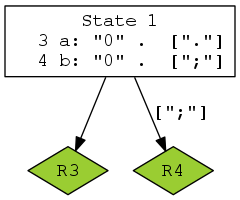
\includegraphics[scale=0.4]{example-reduce}
  \end{center}
\end{frame}

\begin{frame}
  \frametitle{LALR}
  In 1965, Donald Knuth invented the \textbf{LR} parser, which can recognize any
  deterministic context-free language in linear-bounded time. However, rightmost
  derivation has \textbf{very large memory requirements}

  \vfill

  In 1969, Frank DeRemer proposed a simplified version of the LR parser, namely
  the \textbf{Look-Ahead LR} (LALR). The simplification that takes place results
  in a parser with significantly reduced memory requirements but decreased
  language-recognition power. These parsers are seldom written by hand.
\end{frame}

\begin{frame}
  \frametitle{Yet Another Compiler Compiler}
  \textbf{YACC} is an LALR parser generator. It was developed in 1970 by Stephen C.
  Johnson at AT\&T Corporation.

  \vfill

  The \textbf{Berkeley} implementation of Yacc quickly became more popular than
  AT\&T Yacc itself because of lack of reuse restrictions and performance.

  \vfill

  GNU Bison was originally written by Robert Corbett in 1988. Bison was made
  Yacc-compatible by Richard Stallman.

  \vfill

  The \textbf{IEEE POSIX P1003.2} standard defines the functionality and requirements for
  both \texttt{Lex} and \texttt{Yacc}.
\end{frame}

\subsection{Formal grammars}

\begin{frame}
  \frametitle{Syntax}
  The \textbf{syntax} of a computer language is the set of rules that defines
  the combinations of symbols that are considered to be a correctly structured
  document or fragment in that language.

  \vfill

  Syntax – the form – is contrasted with semantics – the meaning.
\end{frame}

\begin{frame}
  \frametitle{Metasyntax}
  A \textbf{metasyntax} describes the allowable structure and composition of
  phrases and sentences of a metalanguage, which is used to describe either a
  natural language or a computer programming language.

  \vfill
  Some of the widely used formal metalanguages for computer languages are
  \textit{Backus–Naur Form} (BNF),
  \textit{Extended Backus–Naur Form} (EBNF), \textit{Wirth syntax notation}
  (WSN), and \textit{Augmented Backus–Naur Form} (ABNF).
\end{frame}

\begin{frame}
  \frametitle{Elements of metasyntax}
  \begin{itemize}
    \item \textbf{Terminals}: a stand-alone syntactic structure. They could be
      denoted by double quoting the name of the terminals.

      E.g. \texttt{“else” , “if”, “then”, “while”}

      \vfill

    \item \textbf{Nonterminals}: a symbolic representation defining a set of
      allowable syntactic structures that is composed of a subset of elements.
      Nonterminals could be denoted by angle bracketing the name of the
      nonterminals.

      E.g. \texttt{<int>, <char>, <boolean>}

      \vfill

    \item \textbf{Metasymbol}: a symbolic representation denoting syntactic
      information.

      E.g. \texttt{:= , |, \{\}, (), [], *}
  \end{itemize}
\end{frame}

\begin{frame}[fragile,shrink=18]
  \frametitle{Backus-Naur Form}
\begin{verbatim}
 <syntax>         ::= <rule> | <rule> <syntax>

 <rule>           ::= <opt-whitespace> "<" <rule-name> ">"
                        <opt-whitespace> "::="
                        <opt-whitespace> <expression> <line-end>

 <opt-whitespace> ::= " " <opt-whitespace> | ""

 <expression>     ::= <list> | <list> "|" <expression>

 <line-end>       ::= <opt-whitespace> <EOL> | <line-end>
                          <line-end>

 <list>           ::= <term> | <term> <opt-whitespace> <list>

 <term>           ::= <literal> | "<" <rule-name> ">"

 <literal>        ::= '"' <text> '"' | "'" <text> "'"
\end{verbatim}
\end{frame}

\begin{frame}[fragile]
  \frametitle{Wirth syntax notation}
  \begin{verbatim}
  SYNTAX     = { PRODUCTION } .
  PRODUCTION = IDENTIFIER "=" EXPRESSION "." .
  EXPRESSION = TERM { "|" TERM } .
  TERM       = FACTOR { FACTOR } .
  FACTOR     = IDENTIFIER
           | LITERAL
           | "[" EXPRESSION "]"
           | "(" EXPRESSION ")"
           | "{" EXPRESSION "}" .
           IDENTIFIER = letter { letter } .
           LITERAL    = """" character { character } """" .
  \end{verbatim}
\end{frame}

\begin{frame}[fragile]
  \frametitle{Extended Backus-Naur Form}
  Derived from regular expressions:
  \begin{itemize}
    \item trailing%vim...
      \texttt{?} means an optional item;
    \item trailing \texttt{+} and \texttt{*} means repeat 1 or more times, or 0
      or more times, respectively.
  \end{itemize}
  \begin{verbatim}
  number = digit+ .
  identifier = letter (letter | digit)* .
  functioncall = functionname "(" parameterlist? ")" .
  \end{verbatim}

  \vfill

  Based on Wirth's definition:
  \begin{itemize}
    \item \texttt{[ ]} means an optional item;
    \item \texttt{\{ \}} means repeat 0 or more times.
  \end{itemize}
  \begin{verbatim}
  number = digit {digit} .
  identifier = letter {letter | digit} .
  functioncall = functionname "(" [parameterlist] ")" .
  \end{verbatim}
\end{frame}

\begin{frame}[fragile]
  \frametitle{Augmented Backus-Naur Form}
  \begin{itemize}
    \item \texttt{[ ]} means an optional item;
    \item leading \texttt{*} means repetition, with optional extra numbers to
      indicate bounds (e.g. \texttt{*} means 0 or more, \texttt{1*} means 1 or
      more, \texttt{2*5} means between two and five times).
  \end{itemize}
  \vfill
  \begin{verbatim}
  number = 1*digit .
  identifier = letter *(letter | digit) .
  functioncall = functionname "(" [parameterlist] ")" .
  \end{verbatim}
\end{frame}

\begin{frame}
  \frametitle{Dangling else problem}
  \begin{itemize}
      \item \texttt{if a then if b then c else d}
      \item To whom does the else belong?
      \item \texttt{if a then (if b then c else d)}
      \item \texttt{if a then (if b then c) else d}
      \item Shift/reduce conflict
    \end{itemize}
\end{frame}

\begin{frame}[fragile]
  \frametitle{Dangling else problem}
\begin{verbatim}
    stmt:
      condition
    | exp

    condition:
      "if" exp "then" stmt
    | "if" exp "then" stmt "else" stmt
\end{verbatim}
\end{frame}

\begin{frame}
  \frametitle{Dangling else problem}
    \begin{itemize}
      \item Precedence solution
      \item \texttt{\%precedence "then"}
      \item \texttt{\%precedence "else"}
    \end{itemize}
\end{frame}

\begin{frame}
  \frametitle{Dangling else problem}
    \begin{itemize}
      \item Associativity solution
      \item \texttt{\%right "then" "else"}
    \end{itemize}
\end{frame}

\begin{frame}
  \frametitle{Dangling else problem}
    \begin{itemize}
      \item Changing the language
      \item \texttt{if a then if b then c fi else d fi}
      \item Often not acceptable
    \end{itemize}
\end{frame}

\section{Getting started}

\begingroup
\setbeamercolor{background canvas}{bg=craneorange!90}
\begin{frame}
    \begin{center}
        \vspace{1cm}
        {\Huge\color{black} \textbf{2.} {\fontencoding{T1}\fontfamily{anttlc}\fontseries{m}\fontshape{n} Getting started}}
    \end{center}
\end{frame}
\endgroup

\begin{frame}
  \frametitle{Grammar}
    \begin{itemize}
      \item Rules
      \item Actions
    \end{itemize}
\end{frame}

\begin{frame}
  \frametitle{Grammar Rules}
    \begin{itemize}
      \item Similar to BNF
      \item No compact way to describe optional elements/lists
      \item Beware of the \texttt{\%empty}!
    \end{itemize}
\end{frame}

\begin{frame}[fragile,shrink=25]
  \frametitle{\texttt{bison/src/parse-gram.y}}
\begin{verbatim}
| "%verbose"                    { report_flag |= report_states; }
| "%yacc"                       { yacc_flag = true; }
| /*FIXME: Err?  What is this horror doing here? */ ";"
;

prologue_declarations:
  %empty
| prologue_declarations prologue_declaration
;

rhses.1:
  rhs                { grammar_current_rule_end (@1); }
| rhses.1 "|" rhs    { grammar_current_rule_end (@3); }
| rhses.1 ";"
;

tag.opt:
  %empty { current_type = NULL; }
| TAG    { current_type = $1; tag_seen = true; }
;
\end{verbatim}
\end{frame}

\begin{frame}[fragile,shrink=25]
  \frametitle{\texttt{bison/tests/named-refs.at}}
\begin{verbatim}
exp:
  NUM                { $$ = $NUM; }
| exp[l] '=' exp[r]
  {
    if ($l != $r)
      fprintf (stderr, "calc: error: %d != %d\n", $l, $r);
   $$ = $l;
  }
| exp[x] '+' { $<ival>$ = $x; } [l] exp[r]  { $$ = $<ival>l + $r;    }
| exp[l] '-' exp[r]  { $$ = $l - $r;        }
| exp[l] '*' exp[r]  { $$ = $l * $r;        }
| exp[l] '/' exp[r]  { $$ = $l / $r;        }
| '-' exp  %prec NEG { $$ = -$2;            }
| exp[l] '^' exp[r]  { $$ = power ($l, $r); }
| '(' exp[e] ')'     { $$ = $e;           }
| '(' error ')'      { $$ = 1111; yyerrok;  }
| '!'                { $$ = 0; YYERROR;     }
| '-' error          { $$ = 0; YYERROR;     }
;
\end{verbatim}
\end{frame}

\begin{frame}[fragile,shrink=25]
  \frametitle{\texttt{lilypond-2.16.2/lily/parser.yy}}
\begin{verbatim}
dots:
  /* empty */   { $$ = 0; }
  | dots '.' { $$ ++; }
  ;
\end{verbatim}
\end{frame}

\begin{frame}[fragile,shrink=25]
  \frametitle{\texttt{bison/tests/actions.at}}
\begin{verbatim}
exp: a_1 a_2 { $<val>$ = 3; } { $<val>$ = $<val>3 + 1; } a_5
     sum_of_the_five_previous_values {
       USE (($1, $2, $<foo>3, $<foo>4, $5));
       printf ("%d\n", $6);
    }
;
a_1: { $$ = 1; };
a_2: { $$ = 2; };
a_5: { $$ = 5; };

sum_of_the_five_previous_values:
    {
       $$ = $<val>0 + $<val>-1 + $<val>-2 + $<val>-3 + $<val>-4;
    }
;

start: one two { $$.val = $1.val + $2.val; } sum ;
one: { $$.val = 1; } ;
two: { $$.val = 2; } ;
sum: { printf ("%d\n", $0.val + $-1.val + $-2.val); } ;
\end{verbatim}
\end{frame}

\begin{frame}[fragile,shrink=25]
  \frametitle{\texttt{postgresql-9.3.2/src/backend/parser/gram.y}}
\begin{verbatim}
      | CREATE CONSTRAINT TRIGGER name AFTER TriggerEvents ON
      qualified_name OptConstrFromTable ConstraintAttributeSpec
      FOR EACH ROW TriggerWhen
      EXECUTE PROCEDURE func_name '(' TriggerFuncArgs ')'
        {
          CreateTrigStmt *n = makeNode(CreateTrigStmt);
          n->trigname = $4;
          n->relation = $8;
          n->funcname = $17;
          n->args = $19;
          n->row = TRUE;
          n->timing = TRIGGER_TYPE_AFTER;
          n->events = intVal(linitial($6));
          n->columns = (List *) lsecond($6);
          n->whenClause = $14;
          n->isconstraint  = TRUE;
          processCASbits($10, @10, "TRIGGER",
                   &n->deferrable, &n->initdeferred, NULL,
                   NULL, yyscanner);
          n->constrrel = $9;
          $$ = (Node *)n;
        }
\end{verbatim}
\end{frame}


\begin{frame}
  \frametitle{Grammar Actions}
    \begin{itemize}
      \item C/C++ code run when the rule is recognized
      \item Create an AST, compute the result of an expression\ldots
      \item Usually at the end
      \item Can be mid-rule actions (lexer context change, \ldots)
    \end{itemize}
\end{frame}

\section{GNU Bison internals}

\begingroup
\setbeamercolor{background canvas}{bg=craneorange!90}
\begin{frame}
    \begin{center}
        \vspace{1cm}
        {\Huge\color{black} \textbf{3.} {\fontencoding{T1}\fontfamily{anttlc}\fontseries{m}\fontshape{n} GNU Bison Internals}}
    \end{center}
\end{frame}
\endgroup

\subsection{Operator Precedence}
\begin{frame}
  \frametitle{A simple model}
    \begin{itemize}
      \item Simple way to represent operator precedence: an int
      \item Increasing order, as precedence increases.
      \item Pro: Simple to understand and to implement
      \item Con: Not very powerful/versatile, can hide errors
    \end{itemize}
\end{frame}

\begin{frame}[fragile]
  \frametitle{Conflict resolution}
\begin{verbatim}
prec(a) > prec(b)?
  -> yes: shift
  -> no: prec(a) < prec(b)?
    -> yes: reduce
    -> no: assoc(a) == ?
      -> %left: reduce
      -> %right: shift
      -> %noassoc: error
      -> nothing/%precedence: conflict
\end{verbatim}
\end{frame}


\begin{frame}
  \frametitle{Moving towards a partial order}
    Objectives:
    \begin{itemize}
      \item To be able to express a partial order on operators
      \item Simple syntax, easily understandable
      \item Clarify grammars, highlight hidden declarations
      \item Retro-compatible
    \end{itemize}
\end{frame}


\begin{frame}
  \frametitle{Proposed solution}
    \begin{itemize}
      \item Group operators by semantics (\texttt{\%gprec \{\}})
      \item Total order inside a group
      \item No comparison possible between groups, by default
      \item Extra instruction to add details (\texttt{\%precr \{\}})
      \item Precedence visualisation tool
    \end{itemize}
\end{frame}

\begin{frame}
  \frametitle{Diagnosis tool}
    \begin{itemize}
      \item Output: \textbf{DOT}
      \item Visualize the precedence relationships
      \item Used, declared, useless...
      \item helps with group identification
    \end{itemize}
\end{frame}

\begin{frame}[fragile]
  \frametitle{Example: Gawk}
  \footnotesize{
  \begin{verbatim}
// From lowest to highest
%right ASSIGNOP ASSIGN SLASH_BEFORE_EQUAL
%right '?' ':'
%left LEX_OR
%left LEX_AND
%left LEX_GETLINE
%nonassoc LEX_IN
%left FUNC_CALL LEX_BUILTIN LEX_LENGTH
%nonassoc ','
%left MATCHOP
%nonassoc RELOP '<' '>' IO_IN IO_OUT
%left CONCAT_OP
%left YSTRING YNUMBER
%left '+' '-'
%left '*' '/' '%'
%right '!' UNARY
%right '^'
%left INCREMENT DECREMENT
%left '$'
%left '(' ')'
\end{verbatim}
}
\end{frame}


\begin{frame}[fragile]
  \frametitle{Example: Gawk}
\begin{verbatim}
%gprec comp_op {
  %precedence ASSIGNOP
  %right '?' ':'
  %left LEX_OR
  %left LEX_AND

  %precedence LEX_IN

  %left MATCHOP
  %nonassoc RELOP '<' '>'
}

\end{verbatim}
\end{frame}

\begin{frame}[fragile]
  \frametitle{Example: Gawk}
\begin{verbatim}
%gprec comp_op {...}
%gprec arith {
  %precedence CONCAT_OP
  %left '+' '-'
  %left '*' '/' '%'
  %precedence UNARY
  %right '^'
}
\end{verbatim}
\end{frame}

\begin{frame}[fragile]
  \frametitle{Example: Gawk}
\begin{verbatim}
%gprec comp_op {...}
%gprec arith {...}

%gprec {
  %precedence LEX_LENGTH
  %precedence '('
}

%precr arith > '<'
\end{verbatim}
\end{frame}

>>>>>>> beamer: operator precedence
\subsection{Wcategories}
\subsection{Homemade variants}
\subsection{GNU M4 backend}

\begin{frame}
\end{frame}

\section{Working with GNU}

\begingroup
\setbeamercolor{background canvas}{bg=craneorange!90}
\begin{frame}
    \begin{center}
        \vspace{1cm}
        {\Huge\color{black} \textbf{4.} {\fontencoding{T1}\fontfamily{anttlc}\fontseries{m}\fontshape{n} Working with GNU}}
    \end{center}
\end{frame}
\endgroup

\subsection{The GNU's habitat}

\begin{frame}
  \begin{center}
    
\includegraphics[scale=0.3]{gnu}
  \end{center}
\end{frame}

\begin{frame}
  \frametitle{The GNU gnulib}
  Suppose you have reusable code:
  \begin{itemize}
    \item likely useful outside your project;
    \item not dependent on your project.
  \end{itemize}
  \vfill
  You can contribute it to the \textbf{gnulib}: a modular source code library,
  composed of:
    \begin{itemize}
      \item \textbf{POSIX} and \textbf{glibc} compatible substitutes;
      \item general purpose code for applications (file system traversal,
        crypto, containers, i18n, etc.);
      \item maintainer infrastructure (\texttt{config.guess}, consistency
        checking tools, upload scripts for \texttt{ftp.gnu.org}, \ldots)
    \end{itemize}
\end{frame}

\begin{frame}[fragile,shrink=25]
  \frametitle{\texttt{gnulib/xmalloc.c}}
\begin{verbatim}
void *
xmalloc (size_t n)
{
  void *p = malloc (n);
  if (!p && n != 0)
    xalloc_die ();
  return p;
}

void *
xcalloc (size_t n, size_t s)
{
  void *p;
  /* Test for overflow, since some calloc implementations don't have
     proper overflow checks.  But omit overflow and size-zero tests if
     HAVE_GNU_CALLOC, since GNU calloc catches overflow and never
     returns NULL if successful.  */
  if ((! HAVE_GNU_CALLOC && xalloc_oversized (n, s))
      || (! (p = calloc (n, s)) && (HAVE_GNU_CALLOC || n != 0)))
    xalloc_die ();
  return p;
}
\end{verbatim}
\end{frame}

\begin{frame}[fragile]
  \frametitle{GNU gettext}
  Wrap strings that the user will see in the \texttt{gettext} function. To reduce code
clutter, it is commonly aliased to \texttt{\_}.

\begin{verbatim}
/// TRANSLATORS: Please leave %s as it is, because it
/// is needed by the program.
printf(_("My name is %s.\n"), my_name);
\end{verbatim}

Then, \texttt{xgettext} is run using the command:

\texttt{xgettext --add-comments=/}

\vfill

The resultant \texttt{.pot} file looks like this with the comment:
\begin{verbatim}
 #. TRANSLATORS: Please leave %s as it is, because it
 # is needed by the program.
 #: src/name.c:36
 msgid "My name is %s.\n"
 msgstr ""
\end{verbatim}
\end{frame}

\begin{frame}[fragile]
  \frametitle{GNU gettext}
The translator derives a \texttt{.po} (Portable Object) file from the template
using the \texttt{msginit} program, then fills out the translations

\begin{verbatim}
msginit --locale=fr --input=name.pot
\end{verbatim}

This will create \texttt{fr.po}.

\begin{verbatim}
 #: src/name.c:36
 msgid "My name is %s.\n"
 msgstr "Je m'appelle %s.\n"
\end{verbatim}
Finally, the \texttt{.po} files are compiled into binary \texttt{.mo} files
with \texttt{msgfmt}.  These are now ready for distribution with the software
package.

The user sets the environment variable \texttt{LC\_MESSAGES}, and the program
will display strings in the selected language.
\end{frame}

\begin{frame}[fragile]
  \frametitle{GNU gettext}
  \begin{center}
    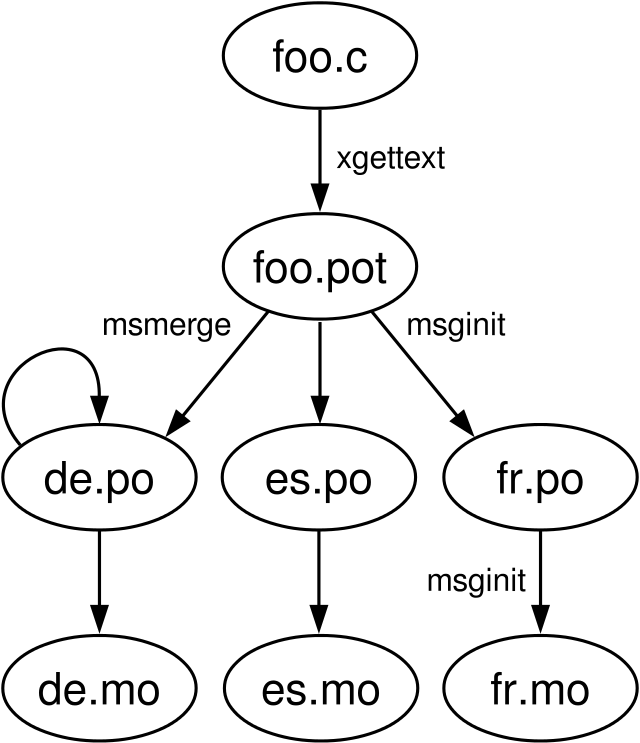
\includegraphics[scale=0.3]{Gettext}
  \end{center}
\end{frame}

\begin{frame}
  \frametitle{obstacks}
It is a memory-management GNU extension. An \textit{obstack} is a
\textbf{stack} of \textit{objects} (data items) which is \textbf{dynamically
managed}. It implements a region-based memory management scheme.

\vfill

Consider reading
\texttt{lrde.epita.fr/$_{\widetilde{~}}$akim/ccmp/doc/gnuprog2/obstack.html}, and
the rest of it too.
\end{frame}

\begin{frame}[fragile]
  \frametitle{obstacks}

Before you can call any of the obstack functions, you need to decide how those
functions will allocate and release dynamic memory, and must define the
following macros in your source file:

\begin{verbatim}
     #define obstack_chunk_alloc  malloc
     #define obstack_chunk_free   free
\end{verbatim}

\vfill

Each function has both a macro definition and a function definition:

\begin{verbatim}
/* Use the macro. */
x = (char *) obstack_alloc(obptr, size);

/* Call the function. */
x = (char *) (obstack_alloc) (obptr, size);
\end{verbatim}
\end{frame}

\begin{frame}[fragile,shrink=25]
  \frametitle{\texttt{bison/src/scan-gram.l}}
\begin{verbatim}
  /*----------------------------.
  | Decode escaped characters.  |
  `----------------------------*/

<SC_ESCAPED_STRING,SC_ESCAPED_CHARACTER>
{
  \\[0-7]{1,3} {
    unsigned long int c = strtoul (yytext + 1, NULL, 8);
    if (!c || UCHAR_MAX < c)
      complain (loc, complaint, _("invalid number after \\-escape: %s"),
                   yytext+1);
    else
      obstack_1grow (&obstack_for_string, c);
  }

  \\x[0-9abcdefABCDEF]+ {
    verify (UCHAR_MAX < ULONG_MAX);
    unsigned long int c = strtoul (yytext + 2, NULL, 16);
    if (!c || UCHAR_MAX < c)
      complain (loc, complaint, _("invalid number after \\-escape: %s"),
                   yytext+1);
    else
      obstack_1grow (&obstack_for_string, c);
  }

  \\a   obstack_1grow (&obstack_for_string, '\a');
  \\b   obstack_1grow (&obstack_for_string, '\b');
\end{verbatim}
\end{frame}

\begin{frame}[fragile,shrink=25]
  \frametitle{\texttt{bison/src/graphviz.c}}
\begin{verbatim}
fprintf (fout, "  %1$d -> \"%1$dR%2$d%3$s\" [",
         source, ruleno, ed);

/* (The lookahead tokens have been added to the beginning of the
   obstack, in the caller function.) */
if (! obstack_empty_p (out))
  {
    char *label = obstack_finish0 (out);
    fprintf (fout, "label=\"[%s]\", ", label);
    obstack_free (out, label);
  }
\end{verbatim}
\ldots
\begin{verbatim}
static bool
print_token (struct obstack *out, bool first, char const *tok)
{
  char const *q = escape (tok);

  if (! first)
    obstack_sgrow (out, ", ");
  obstack_sgrow (out, q);
  return false;
}
\end{verbatim}
\end{frame}

\begin{frame}[fragile,shrink=25]
  \frametitle{\texttt{gnulib/lib/obstack.h}}
\begin{verbatim}
/* Similar to _BPTR_ALIGN (B, P, A), except optimize the common case
   where pointers can be converted to integers, aligned as integers,
   and converted back again.  If PTR_INT_TYPE is narrower than a
   pointer (e.g., the AS/400), play it safe and compute the alignment
   relative to B.  Otherwise, use the faster strategy of computing the
   alignment relative to 0.  */

#define __PTR_ALIGN(B, P, A)                                                \
  __BPTR_ALIGN (sizeof (PTR_INT_TYPE) < sizeof (void *) ? (B) : (char *) 0, \
                P, A)

...
#define obstack_alignment_mask(h) ((h)->alignment_mask)

/* To prevent prototype warnings provide complete argument list.  */
#define obstack_init(h)                                         \
  _obstack_begin ((h), 0, 0,                                    \
                  (void *(*) (long)) obstack_chunk_alloc,       \
                  (void (*) (void *)) obstack_chunk_free)
...
# define obstack_1grow(OBSTACK,datum)                                   \
__extension__                                                           \
({ struct obstack *__o = (OBSTACK);                                     \
   if (__o->next_free + 1 > __o->chunk_limit)                           \
     _obstack_newchunk (__o, 1);                                        \
   obstack_1grow_fast (__o, datum);                                     \
   (void) 0; })
\end{verbatim}
\end{frame}

\subsection{The GNU world}

\begin{frame}
  \frametitle{Contributing}
    \begin{itemize}
      \item Open source
      \item Peer review (quality standards)
      \item Testsuite
      \item Patches (e-mail)
    \end{itemize}
\end{frame}

\begin{frame}
  \frametitle{Coding style}
    \begin{itemize}
      \item GNU prototyping convention
      \item Recently switched from ansi C89 to C99
      \item Indentation
      \item Comments (nice format)
      \item Clean code
    \end{itemize}
\end{frame}

\begin{frame}
  \frametitle{Git}
    \begin{itemize}
      \item Commit early, commit often
      \item Every commit passes the testsuite (and compiles, of course!)
      \item A bugfix comes with a test
      \item Patch, integrated by the maintainers (Akim)
      \item String commit formatting
    \end{itemize}
\end{frame}

\begin{frame}
  \frametitle{Testsuite}
    \begin{itemize}
      \item m4 macros
      \item Not unit-tests
      \item TESTSUITEFLAGS (specific tests, threading, \ldots)
      \item Testsuite needs to be compiled
    \end{itemize}
\end{frame}

\end{document}
